\documentclass[runningheads]{llncs}
\usepackage[ruled]{algorithm2e}
\usepackage{amsfonts}
\usepackage{amsmath}
\usepackage{bm}
\usepackage{booktabs}
\usepackage{color}
\usepackage[compress]{cite}
\usepackage{graphicx}
\usepackage{hyperref}
\usepackage{lscape}
\usepackage{multirow}
\usepackage{physics}

\renewcommand\UrlFont{\color{blue}\rmfamily}
\SetKwInput{KwHyperparameters}{Hyperparameters}
\SetKwInput{KwInput}{Input}
\SetKwInput{KwOutput}{Output}
\SetKwComment{Comment}{/* }{ */}
\DeclareMathOperator{\sgn}{sgn}
\DeclareMathOperator*{\argmax}{arg\,max}
\setlength{\tabcolsep}{7pt}
\newtheorem{prop}{Proposition}

\begin{document}

\title{
  The Ticket Restaurant Assignment Problem
}
\author{Gabriele Cerizza}
\authorrunning{G. Cerizza}

\institute{Università degli Studi di Milano\\
\email{gabriele.cerizza@studenti.unimi.it}\\
\url{https://github.com/gabrielecerizza/orc_project}}

\maketitle

\section*{Introduction}
\label{sec:introduction}

In this report we detail a branch-and-bound exact algorithm based on Lagrangean relaxation to solve the ticket restaurant assignment problem (TRAP), pursuant to the project specifications set out for the Operational Research Complements course of the Università degli Studi di Milano\footnote{\url{https://homes.di.unimi.it/righini/Didattica/ComplementiRicercaOperativa/ComplementiRicercaOperativa.htm}}. 

In Section~\ref{sec:problem} we define the problem. In Section~\ref{sec:branch-bound} we describe the main aspects of the branch-and-bound algorithm. In Section~\ref{sec:results} we show the results of our experiments. Finally, Section~\ref{sec:conclusions} contains our concluding remarks.

\section{Ticket Restaurant Assignment Problem}
\label{sec:problem}

In this section we define the TRAP (Section~\ref{subsec:problem:definition}), we formalize it as a mathematical programming problem (Section~\ref{subsec:problem:formalization}) and we examine the relevant literature (Section~\ref{subsec:problem:related_works}).

\subsection{Definition}
\label{subsec:problem:definition}

The TRAP is defined as follows. A ticket company possesses two kinds of restaurant tickets: the low-profit tickets and the high-profit tickets. The ticket company gives the tickets to customer companies. Each customer company receives only one kind of tickets and distributes the tickets to its employees, who use them to buy meals in a given set of restaurants.

For each restaurant a given ratio between low-profit and high-profit tickets must be observed. 
The ticket company must maximize the profit while complying with this constraint. Thus, maximizing the profit amounts to minimizing the number of low-profit tickets while ensuring that a given amount of low-profit tickets is assigned for each considered restaurant.

\subsection{Formalization}
\label{subsec:problem:formalization}

Let $I = \{1,\dots,m\}$ be a set of restaurants, $J = \{1,\dots,n\}$ be a set of customer companies, $b \in \mathbb{Z}_{+}^{m}$ be the vector representing the minimum amount of low-profit tickets to be used for each restaurant, and $A \in \mathbb{Z}_{+}^{m \times n}$ be the matrix representing the amount of low-profit tickets, assigned to each customer company, that are used in each restaurant. Therefore, $a_{ij}$ is the amount of low-profit tickets, assigned to customer company $j$, that are used in restaurant $i$. Then, the integer linear programming model of the TRAP is the following:
\begin{alignat}{3}
  &\min & \quad & z = \sum_{j \in J} \left( \sum_{i \in I} a_{ij} \right) x_j \label{eq:primal}\\
  &\text{subject to}  &       & \sum_{j \in J} a_{ij} x_j \ge b_i & \qquad & i = 1,\dots,m \, , \notag\\
  &                   &       & x_j \in \{0,1\}  &\qquad& j = 1,\dots,n \, , \notag
\end{alignat}
where each binary variable $x_j$ indicates whether customer company $j$ is assigned low-profit tickets. A cover is a vector $x$ such that $Ax \ge b$.

From (\ref{eq:primal}), the following Lagrangean relaxation (LR) is obtained:
\begin{alignat}{3}
  &\min & \quad & z_{\text{LR}} = \sum_{j \in J} \left( \sum_{i \in I} (1 - \lambda_i) a_{ij} \right) x_j + \sum_{i \in I} \lambda_i b_i \label{eq:lagrangean}\\
  &\text{subject to}  &       & x_j \in \{0,1\} & \qquad & j = 1,\dots,n \, , \notag\\
  &                   &       & \lambda_i \ge 0  & \qquad & i = 1,\dots,m \, , \notag
\end{alignat}
where $\lambda_i$ are the Lagrangean multipliers.

The TRAP is a generalization of the set covering problem (SCP), as explained in the following section. The SCP is NP-hard~\cite{caprara-2000-algorithms}, hence so is the TRAP.

\subsection{Related Works}
\label{subsec:problem:related_works}

\subsubsection{Set covering problem.} The problem at hand is equivalent to the SCP when $A$ is a binary matrix and $b$ is an all-ones vector. The SCP has been treated extensively in literature and the ideas developed in that context can be leveraged to solve the TRAP. For the SCP, both exact and heuristic algorithms have been devised (see the survey in~\cite{caprara-2000-algorithms}). We focus only on exact algorithms for our problem. 

% However, we stress that large-scale problem instances involving millions of variables and thousands of constraints may be tackled only by heuristic approaches, as observed in~\cite{ceria-1998-lagrangian,caprara-1999-lagrangian}.

The following works in the field of SCP are of particular interest to us. Balas and Ho~\cite{balas-ho-2009-set-covering} adopted a branch-and-cut algorithm, comprising a primal heuristic to find upper bounds and subgradient optimization to find lower bounds.
Beasley~\cite{beasley-1987-algorithm} adopted a branch-and-bound algorithm, computing upper bounds with a greedy heuristic, computing lower bounds with dual ascent and subgradient optimization, and devising problem reduction techniques.
Balas and Carrera~\cite{balas-carrera-1996-dynamic} adopted a dynamic subgradient-based branch-and-bound algorithm, additionally employing variable fixing techniques and heuristics to obtain upper bounds.

We fashioned our branch-and-bound algorithm based on the algorithms described in these works, adapting their solutions to account for the distinctive features of the TRAP. In particular, these distinctive features preclude the use of techniques relying on the fact that each constraint can be satisfied by setting to 1 exactly one variable with a non-zero coefficient in the row corresponding to that constraint.

\subsubsection{Multicovering problem.} A problem closely related to the TRAP is the one called multicovering problem (MCP)~\cite{hall-hochbaum-1986-fast-approximation, hall-hochbaum-1992-multicovering}, defined as follows:
\begin{alignat}{3}
  &\min & \quad & z = c^\top x \notag\\
  &\text{subject to}  &       & Ax \ge b \, , \notag\\
  &                   &       & x_j \in \{0, 1\}  & \qquad & \forall j=1,\dots,n \, , \notag
\end{alignat}
where $A$ is a binary matrix and $b$ is a vector of positive integers. This problem differs from the one at hand in that $A$ is binary and not simply non-negative.

Notably, Hall and Hochbaum~\cite{hall-hochbaum-1992-multicovering} adopted a branch-and-cut procedure to solve the MCP, using a primal heuristic to find upper bounds and combining a dual heuristic with subgradient optimization to find lower bounds. From this work we derived the main primal heuristic for our branch-and-bound algorithm (see Sections~\ref{subsec:branch-bound:primal} and~\ref{subsec:results:comparisons}). 

\subsubsection{Covering integer problem.} Finally, a generalization of the TRAP is given by the so-called covering integer problem (CIP)~\cite{kolliopoulos-2003-approximating,kolliopoulos-2005-approximation}, defined as follows:
\begin{alignat}{3}
  &\min & \quad & z = c^\top x \notag\\
  &\text{subject to}  &       & Ax \ge b \, , \notag\\
  &                   &       & x_j \le d_j & \qquad & \forall j=1,\dots,n \, , \notag\\
  &                   &       & x_j \in \mathbb{Z}_{+}  & \qquad &  \forall j=1,\dots,n \, , \notag
\end{alignat}
where all the entries in $A$, $b$, $c$ and $d$ are non-negative. This problem is equivalent to the TRAP when $d_j = 1$ for all $j=1,\dots,n$. Unfortunately, we found only approximation algorithms for the CIP (see~\cite{kolliopoulos-2003-approximating,kolliopoulos-2005-approximation}).

\section{Branch-and-Bound}
\label{sec:branch-bound}

In this section we describe the different aspects of the branch-and-bound algorithm employed to solve the TRAP: the primal heuristics used to find upper bounds (Section~\ref{subsec:branch-bound:primal}); the strategies used to find lower bounds (Section~\ref{subsec:branch-bound:lb}); the branching rules (Section~\ref{subsec:branch-bound:branch}); and the reduction techniques (Section~\ref{subsec:branch-bound:reduction}). 

\subsection{Primal Heuristics}
\label{subsec:branch-bound:primal}

\subsubsection{Greedy heuristic.} This heuristic selects greedily the variables of the cover, picking the row $i$ with the largest ratio $\frac{\sum_{j \in J} a_{ij}}{b_i}$ and then picking the column with the largest coefficient. Each time a variable is selected, the coefficients on the left-hand side (LHS) and right-hand side (RHS) are decreased accordingly.

This heuristic selects the row which is easiest to cover, since a larger ratio means that more solutions might satisfy the constraint. Indeed, when $\sum_{j \in J} a_{ij} = b_i$, we must select all variables with non-zero entries in $A_i$ in order to satisfy the constraint, thus restricting the number of possible solutions. By picking the column with the largest coefficient we aim to satisfy the constraint in the fastest way.

\subsubsection{Dobson heuristic.} This heuristic is taken from Dobson~\cite{dobson-1982-worst-case} and generalizes an heuristic for the SCP from Chvatal~\cite{chvatal-1979-greedy}. This heuristic picks the column $j$ that minimizes $c_j \sum_{i \in I} a_{ij}$. Furthermore, any $a_{ij}$ larger than $b_i$ is lowered down to $b_i$.

The idea of this heuristic is to pick the column that covers the most while costing the least. In the case of the TRAP, however, the cost of each column is equal to the sum of the coefficients of that column, which means that all columns could be equivalently selected. The only exception occurs when $\exists i \in I, j \in J : a_{ij} > b_i$. In this case, $a_{ij}$ would be lowered and therefore $c_j \sum_{i \in I} a_{ij}$ would also be lowered. Therefore, this heuristic, when applied to the TRAP, prioritizes the columns whose coefficients are more than enough to cover the remaining part of $b_i$ for any $i$. 

\subsubsection{Hall-Hochbaum heuristic.} This heuristic adapts one of the heuristics conceived by Hall and Hochbaum~\cite{hall-hochbaum-1992-multicovering}. Specifically, this heuristic picks the column $j$ that maximizes $\frac{1}{c_j} \sum_{i \in L} \frac{b_i a_{ij}}{\text{space}(i)}$, where $L = \{i \in I : b_i > 0 \}$ and $\text{space}(i) = \sum_{j \in J} a_{ij} - b_i$.

\subsection{Lower Bounds}
\label{subsec:branch-bound:lb}

\subsubsection{Lagrangean relaxation.} A lower bound to the optimal value of problem~(\ref{eq:primal}) can be obtained by solving the LR defined in~(\ref{eq:lagrangean}). When the Lagrangean multipliers $\lambda$ are given, the objective function of~(\ref{eq:lagrangean}) is trivially minimized by setting $x_j$ to 1 when $\sum_{i \in I} (1 - \lambda_i) a_{ij} < 0$ and to 0 otherwise. The only problem left is to find the optimal Lagrangean multipliers, which yield the highest lower bound.

Subgradient optimization is a popular algorithm to find the optimal Lagrangean multipliers. Our version of subgradient optimization is adapted from~\cite{balas-carrera-1996-dynamic} and is described in Algorithm~\ref{alg:subgrad}, where $z_{\text{UB}}$ is the best incumbent upper bound and $z_{\text{LB}}$ is the lower bound.

\begin{algorithm}
  \DontPrintSemicolon
  \caption{Subgradient optimization}\label{alg:subgrad}
  \KwInput{$A$, $b$, $z_{\text{UB}}$; $f$, $k$, $\epsilon$, $\omega$}
  $t \gets 1$\; 
  $\lambda_i^t = 0 ~ \forall i \in I$\;
  $\lambda_{\text{best}} \gets \lambda^t$\;
  $z_{\text{LB}} \gets 0$\; 
  $z_{\text{best}} \gets z_{\text{LB}}$\; 
  \While{$z_{\text{UB}} > z_{\text{LB}}$ }{
    \For{$j \in J$}{
      \eIf{$\sum_{i \in I} (1 - \lambda^t_i) a_{ij} < 0$}{
        $x_j \gets 1$
      }
      {
        $x_j \gets 0$
      }
    }
    $L(\lambda^t) \gets \sum_{j \in J} \left( \sum_{i \in I} (1 - \lambda^t_i) a_{ij} \right) x_j + \sum_{i \in I} \lambda^t_i b_i$\;
    \If{$L(\lambda^t) > z_{\text{LB}}$}{
      $z_{\text{LB}} \gets L(\lambda^t)$\;
      $z_{\text{best}} \gets z_{\text{LB}}$\;
      $\lambda_{\text{best}} \gets \lambda^t$\;
    }
    $g(\lambda^t) \gets b - Ax$\;
    \If{$z_{\text{LB}}$ unchanged for $k$ iterations}{
      $f \gets \frac{f}{2}$\; 
    }
    $\sigma^t \gets \frac{f(z_{\text{UB}} - z_{\text{LB}})}{\norm{g(\lambda^t)}^2}$\;
    \For{$i \in I$}{
      $\lambda_i^{t+1} \gets \max(0, \lambda_i^t + \sigma^t g_i(\lambda^t))$
    }
    $t \gets t + 1$\;
    \If{$f < \epsilon \lor t > \omega$}{break}
  }
  \Return $z_{\text{best}}$, $\lambda_{\text{best}}$
\end{algorithm}

We cannot assume that the optimal Lagrangean multipliers can be confined within the range $[0, 1]$.

\begin{prop}
  The optimal Lagrangean multipliers for problem~(\ref{eq:lagrangean}) may not lie in the range $[0, 1]$.
\end{prop}

\begin{proof}
  Consider a matrix $A = \begin{bmatrix}
    1 & 2 & 3\\
    3 & 1 & 4\\
    2 & 2 & 2
    \end{bmatrix}$ and a vector $b = \begin{bmatrix}2\\5\\1\end{bmatrix}$. If we run Algorithm~\ref{alg:subgrad} with parameters $f=2$, $k=5$, $\epsilon=0.005$, $\omega=150$ and we bind the Lagrangean multipliers in the range $[0, 1]$, we obtain $z_{\text{LB}} = 8$ and $\lambda = \begin{bmatrix}1\\1\\1\end{bmatrix}$. Running the algorithm with the same parameters, but without bounds on the Lagrangean multipliers, we obtain $z_{\text{LB}} = 10.498$ and $\lambda = \begin{bmatrix}0\\2.259\\0\end{bmatrix}$. \hfill $\square$
\end{proof}

\subsubsection{LP relaxation.} Finally, one could consider solving the LP relaxation of~(\ref{eq:primal}) to obtain a lower bound. In fact, it is observed in~\cite{caprara-2000-algorithms} that ``the lower bound determined by Lagrangian or alternative relaxations is much worse than the optimal solution value of the LP relaxation". The same Authors remark that exact algorithms behave better with LP relaxation, whereas Lagrangean relaxation is better suited for heuristic algorithms.   

\subsection{Branching Rules}
\label{subsec:branch-bound:branch}

\subsubsection{Reduced costs branching.} For this branching rule we compute the reduced costs $r$ of the variables with the formula $r = (1 - \lambda) \cdot A$. After that, we determine a solution by setting to 0 all the variables not fixed to 1 in the current node. Considering the computed solution, we select the variable $x_j$ with the minimum reduced cost and a non-zero coefficient in the row with the largest violation. Finally, we generate two children nodes, fixing $x_j = 0$ in the first node and $x_j = 1$ in the second.

\subsubsection{Costs branching for LP.} This branching rule differs from the reduced costs branching rule only because it selects the variable with the minimum cost instead of the variable with the minimum reduced cost. This modification allows to employ this rule with the LP relaxation, since in that case we do not have the Lagrangean multipliers (or dual variables) $\lambda$. 

\subsubsection{Beasley branching.} This is the branching rule used in~\cite{beasley-1987-algorithm} and differs from the reduced costs branching rule only because it selects the row whose corresponding Lagrangean multiplier has the largest value instead of the row with the largest violation.

\subsection{Reduction}
\label{subsec:branch-bound:reduction}

\subsubsection{Lagrangean penalties.} Following~\cite{beasley-1987-algorithm}, we use the reduced costs to fix variables to 0 or to 1, thus reducing the size of the problem instances. 

Let $r = (1 - \lambda) \cdot A$ be the vector of reduced costs, $z_{\text{LB}}$ be the lower bound of the current node and $z_{\text{UB}}$ be the best incumbent upper bound. Then we can fix $x_j$ to 0 when $r_j \ge 0$ and $z_{\text{LB}} + r_j > z_{\text{UB}}$, and we can fix $x_j$ to 1 when $r_j < 0$ and $z_{\text{LB}} - r_j > z_{\text{UB}}$.  

\subsubsection{Column inclusion.} This reduction method is adapted from~\cite{beasley-1987-algorithm} and consists in fixing to 1 all the free variables with a non-zero coefficient in an uncovered row, when said row cannot be covered otherwise.

\section{Computational Results}
\label{sec:results}

In this section we describe the machine and the technologies used to run the experiments (Section~\ref{subsec:results:tech}), we illustrate how the TRAP instances are generated (Section~\ref{subsec:results:generation}), and then we show the results of our tests (Section~\ref{subsec:results:comparisons}).  

\subsection{Hardware and Technologies}
\label{subsec:results:tech}

We ran the branch-and-bound algorithm on a machine with 16 gigabytes of RAM and a CPU Intel(R) Core(TM) i7-9700K 3.60GHz with 8 cores. The code was implemented in Python 3.11.2.

We include in our comparisons the results obtained with a state-of-the-art commercial solver, Gurobi 10.0.2\footnote{https://www.gurobi.com/}. Note that Gurobi, unlike our implementation, exploits multi-threading. 

% Moreover, the Gurobi engine is written in C and is therefore faster than plain Python code. These factors should be taken into account when evaluating the results.    

\subsection{Problem Generation}
\label{subsec:results:generation}

We generate random TRAP instances by determining the number of constraints ($m$) and variables ($n$) and the density of the problem. The density is the percentage of non-zero coefficients in each row of the matrix $A$.

For each row, we pick the value of $b_i$ uniformly at random between $n$ and $n^2$. After that, the sum of the coefficients on the LHS is picked uniformly at random between $2b_i$ and $5b_i$. Then, we determine the number of columns with a non-zero coefficient using the density parameter, selecting their indices uniformly at random. Finally, the sum of the coefficients on the LHS is distributed uniformly at random among the selected column indices.

\subsection{Comparative Analysis}
\label{subsec:results:comparisons}

\subsubsection{Primal heuristics.} Table~\ref{tab:results:primal} compares the lower bounds obtained by the different primal heuristics described in Section~\ref{subsec:branch-bound:primal} over sets of randomly generated TRAP instances with different numbers of rows and columns. We observe that the bigger is the size of the problem instance, the more the Hall-Hochbaum heuristic outperforms the other primal heuristics. For this reason, only this heuristic was employed in the subsequent experiments. 

\begin{table}
  \caption{Number of times each primal heuristic provided the solution with the lowest upper bound over sets of 10 randomly generated TRAP instances with different numbers of rows and columns and with density equal to $0.5$. The best result for each set of problem instances is highlighted in bold.}
  \label{tab:results:primal}
  \centering
  \begin{tabular}{llccc}
    \toprule
     &  & Greedy & Dobson & Hall-Hochbaum \\
    Rows & Columns &  &  &  \\
    \midrule
    5 & 10 & 1 & \bfseries 7 & 2 \\
    10 & 20 & 1 & 3 & \bfseries 6 \\
    20 & 50 & 0 & 0 & \bfseries 10 \\
    50 & 100 & 0 & 0 & \bfseries 10 \\
    \bottomrule
    \end{tabular}
  \end{table}

\subsubsection{Subgradient optimization parameters.} We set the subgradient optimization parameters as: $f=2$, $k=5$, $\epsilon=0.005$, $\omega=150$. Setting $\omega=150$ allows to achieve a lower bound with at most a $0.016\%$ gap with respect to the optimal lower bound for problems having up to 50 rows and up to 60 columns, as shown in Figure~\ref{fig:results:subgrad}.

\begin{figure}
  \center
  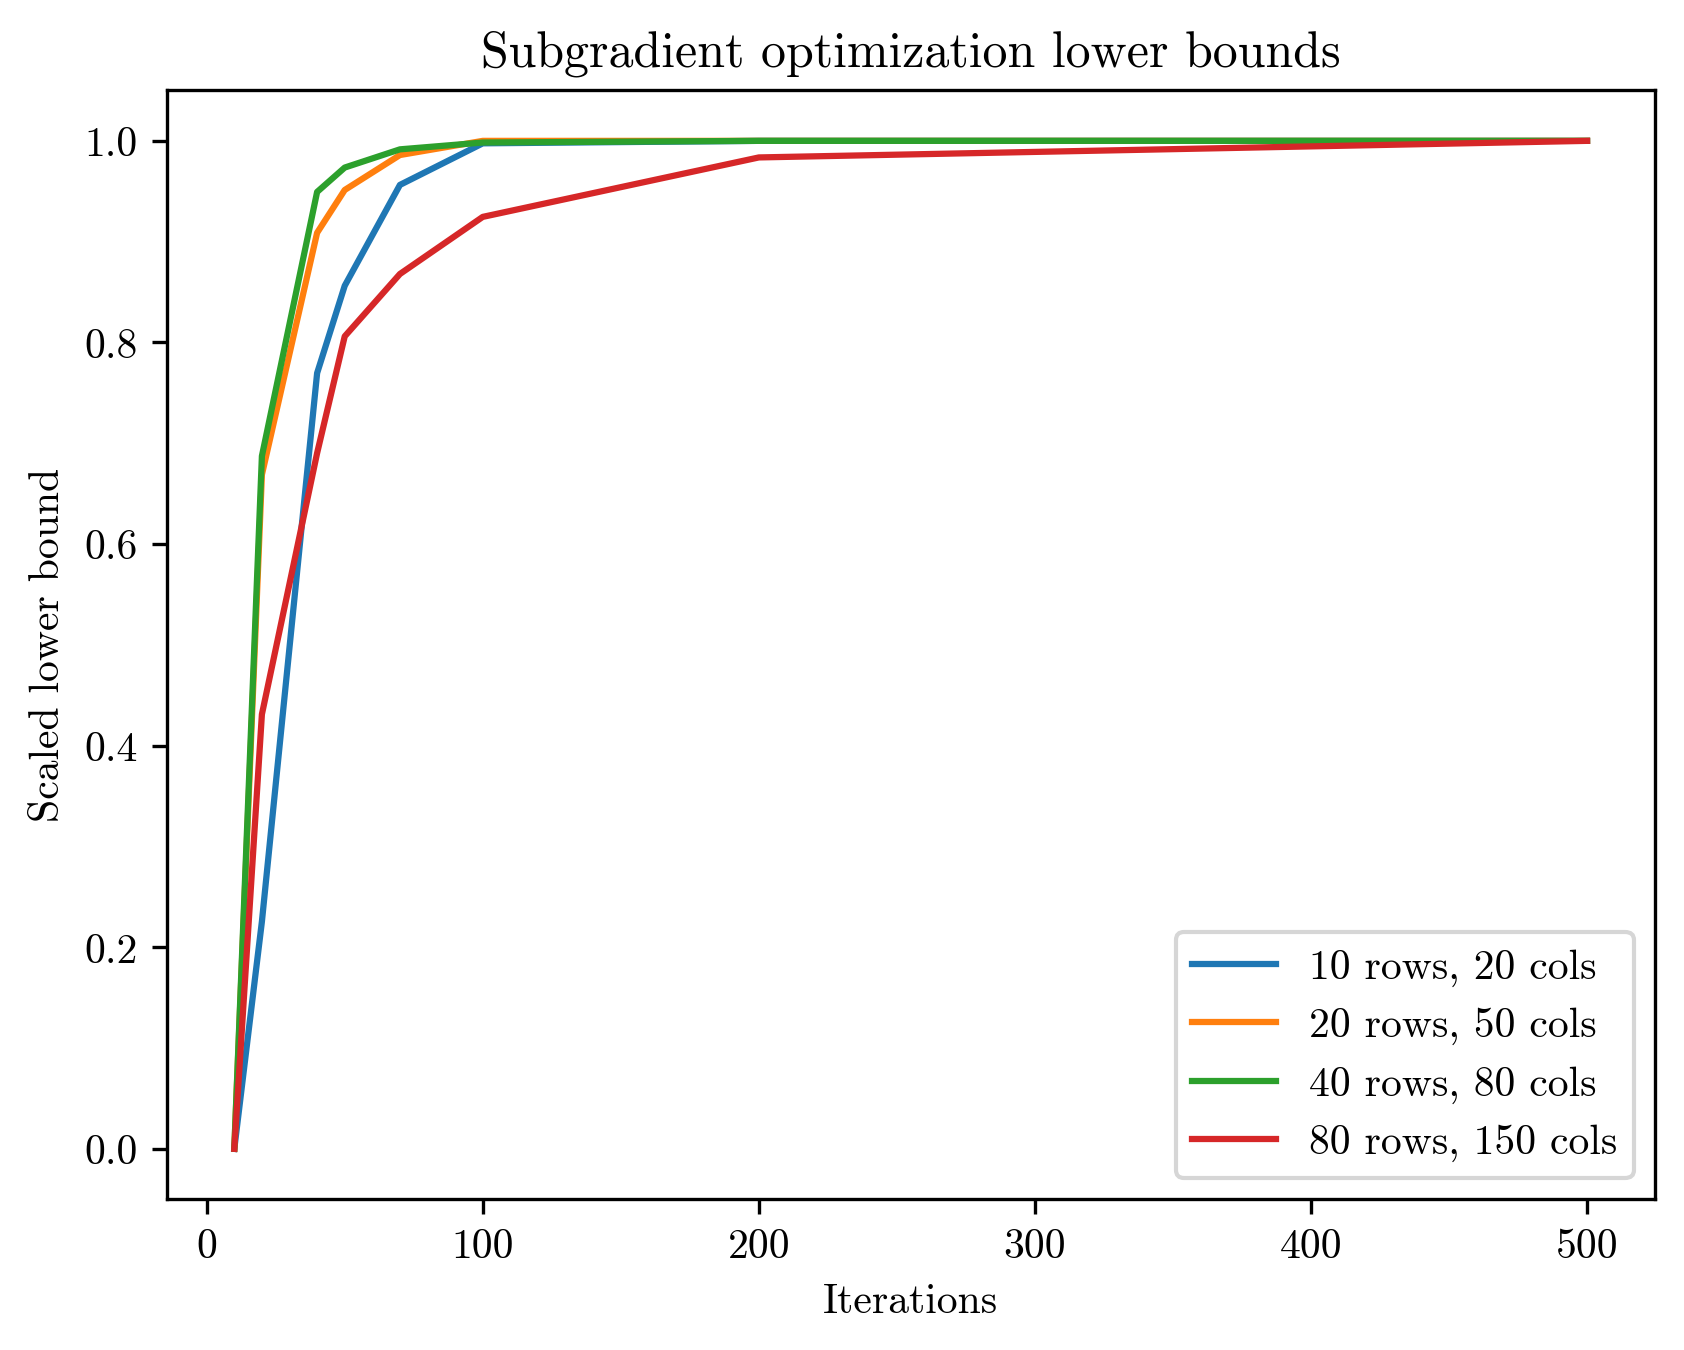
\includegraphics[width=0.7\textwidth]{img/subgrad_lb.png}
  \caption{Min-max scaled lower bounds obtained with subgradient optimization for different numbers of iterations (parameter $\omega$) averaged over sets of randomly generated TRAP instances with different numbers of rows and columns and with density equal to 0.5. Each set contained 10 problem instances.} 
  \label{fig:results:subgrad}
\end{figure}

\subsubsection{Runtime and number of nodes.} We compare different configurations for the branch-and-bound algorithm:
\begin{itemize}
  \item S: reduced costs branching rule and subgradient optimization lower bound, without any primal heuristic and without any reduction technique;
  \item SP: same as S but with Hall-Hochbaum primal heuristic;
  \item SPR: same as SP but with both the reduction techniques described in Section~\ref{subsec:branch-bound:reduction};
  \item SPRR: same as SPR but with the primal heuristic executed only at the root node;
  \item SPRB: same as SPR but with Beasly branching rule instead of reduced costs branching rule;
  \item LP: costs branching rule, LP relaxation lower bound, Hall-Hochbaum primal heuristic and column inclusion reduction technique.
\end{itemize}

Tables~\ref{tab:results:runtime} and~\ref{tab:results:nodes} respectively give the runtime and number of nodes for each of these configurations over randomly generated TRAP instances. We forcibly terminated the algorithm when the runtime exceeded 5 minutes. 

Table~\ref{tab:results:runtime} shows how SPR, SPRR and SPRB achieve similar results and outperform the other configurations for all problem instances. Table~\ref{tab:results:nodes} confirms these results and also reveals how the Beasly branching rule is marginally better than the reduced costs branching rule as far as the number of nodes is concerned. Contrary to what was observed in Section~\ref{subsec:branch-bound:lb}, LP yields the worst results for most problem instances. 

All this considered, the algorithm still performs poorly when compared to Gurobi. A look at the logs of Gurobi reveals that the solver employs a branch-and-cut algorithm, performing root relaxation and finding heuristic solutions periodically. Some of the mentioned cuts are: Gomory, Cover, MIR, StrongCG, Mod-K, Zero half, RLT.

\begin{table}
  \caption{Runtime of different configurations of the branch-and-bound algorithm over randomly generated TRAP instances with different numbers of rows and columns and different densities. Configurations whose runtime exceeded 5 minutes were assigned nan values. The best result obtained by algorithms other than Gurobi is highlighted in bold for each problem instance. The runtime was measured in seconds.}
  \label{tab:results:runtime}
  \centering
  \resizebox{1\textwidth}{!}{
    \begin{tabular}{lllccccccc}
      \toprule
       &  &  & Gurobi & S & SP & SPR & SPRR & SPRB & LP \\
      Rows & Columns & Density &  &  &  &  &  &  &  \\
      \midrule
      \multirow[c]{3}{*}{5} & \multirow[c]{3}{*}{10} & 0.3 & 0.02 & \bfseries 0.00 & \bfseries 0.00 & \bfseries 0.00 & \bfseries 0.00 & \bfseries 0.00 & \bfseries 0.00 \\
       &  & 0.5 & 0.00 & \bfseries 0.09 & 0.17 & 0.14 & 0.12 & 0.14 & 0.11 \\
       &  & 0.7 & 0.00 & 0.02 & 0.06 & 0.03 & \bfseries 0.00 & 0.02 & 0.19 \\
      \cline{1-10}
      \multirow[c]{3}{*}{10} & \multirow[c]{3}{*}{20} & 0.3 & 0.00 & 11.47 & 14.58 & 3.88 & \bfseries 3.06 & \bfseries 3.06 & 39.77 \\
       &  & 0.5 & 0.02 & 23.44 & 24.75 & 5.72 & \bfseries 4.84 & 5.22 & 83.11 \\
       &  & 0.7 & 0.03 & 19.81 & 18.69 & 1.95 & \bfseries 1.86 & \bfseries 1.86 & 165.83 \\
      \cline{1-10}
      \multirow[c]{3}{*}{13} & \multirow[c]{3}{*}{22} & 0.3 & 0.02 & 42.72 & 49.08 & 6.75 & 6.47 & \bfseries 2.62 & 94.09 \\
       &  & 0.5 & 0.00 & 16.12 & 19.83 & 2.98 & 2.80 & \bfseries 2.45 & nan \\
       &  & 0.7 & 0.02 & 28.42 & 28.73 & \bfseries 1.31 & 1.50 & 1.33 & nan \\
      \cline{1-10}
      \multirow[c]{3}{*}{15} & \multirow[c]{3}{*}{25} & 0.3 & 0.00 & 19.08 & 23.19 & 5.38 & 5.69 & \bfseries 2.75 & nan \\
       &  & 0.5 & 0.02 & 28.47 & 29.22 & 5.08 & \bfseries 3.77 & 4.33 & nan \\
       &  & 0.7 & 0.05 & 84.94 & 100.38 & 15.56 & \bfseries 13.75 & 15.64 & nan \\
      \cline{1-10}
      \multirow[c]{3}{*}{20} & \multirow[c]{3}{*}{40} & 0.3 & 0.03 & nan & nan & nan & nan & nan & nan \\
       &  & 0.5 & 0.38 & nan & nan & nan & nan & \bfseries 253.97 & nan \\
       &  & 0.7 & 0.31 & nan & nan & nan & nan & nan & nan \\
      \bottomrule
      \end{tabular}
  }
\end{table}

\begin{table}
  \caption{Number of nodes generated by different configurations of the branch-and-bound algorithm over randomly generated TRAP instances with different numbers of rows and columns and different densities. Configurations whose runtime exceeded 5 minutes were assigned nan values. The best result obtained by algorithms other than Gurobi is highlighted in bold for each problem instance.}
  \label{tab:results:nodes}
  \centering
  \resizebox{1\textwidth}{!}{
    \begin{tabular}{lllccccccc}
      \toprule
       &  &  & Gurobi & S & SP & SPR & SPRR & SPRB & LP \\
      Rows & Columns & Density &  &  &  &  &  &  &  \\
      \midrule
      \multirow[c]{3}{*}{5} & \multirow[c]{3}{*}{10} & 0.3 & 0 & 17 & 15 & \bfseries 5 & \bfseries 5 & 7 & 23 \\
       &  & 0.5 & 1 & 179 & 185 & \bfseries 63 & \bfseries 63 & \bfseries 63 & 183 \\
       &  & 0.7 & 1 & 75 & 85 & \bfseries 23 & \bfseries 23 & \bfseries 23 & 323 \\
      \cline{1-10}
      \multirow[c]{3}{*}{10} & \multirow[c]{3}{*}{20} & 0.3 & 1 & 9131 & 8659 & 1607 & 1761 & \bfseries 1205 & 55541 \\
       &  & 0.5 & 50 & 15421 & 14115 & 2469 & 2781 & \bfseries 2337 & 124795 \\
       &  & 0.7 & 25 & 14057 & 8705 & 609 & 607 & \bfseries 559 & 209799 \\
      \cline{1-10}
      \multirow[c]{3}{*}{13} & \multirow[c]{3}{*}{22} & 0.3 & 1 & 25257 & 26033 & 2427 & 2849 & \bfseries 907 & 117271 \\
       &  & 0.5 & 1 & 9147 & 8837 & 949 & 951 & \bfseries 795 & nan \\
       &  & 0.7 & 1 & 18929 & 14419 & \bfseries 371 & 501 & 453 & nan \\
      \cline{1-10}
      \multirow[c]{3}{*}{15} & \multirow[c]{3}{*}{25} & 0.3 & 1 & 13387 & 13475 & 1631 & 2077 & \bfseries 833 & nan \\
       &  & 0.5 & 59 & 15903 & 14897 & 1731 & 1657 & \bfseries 1541 & nan \\
       &  & 0.7 & 384 & 53149 & 50545 & \bfseries 4549 & 5315 & 4841 & nan \\
      \cline{1-10}
      \multirow[c]{3}{*}{20} & \multirow[c]{3}{*}{40} & 0.3 & 174 & nan & nan & nan & nan & nan & nan \\
       &  & 0.5 & 573 & nan & nan & nan & nan & \bfseries 62615 & nan \\
       &  & 0.7 & 1865 & nan & nan & nan & nan & nan & nan \\
      \bottomrule
      \end{tabular}
  }
\end{table}

\section{Conclusions}
\label{sec:conclusions}

In this work we described and evaluated a branch-and-bound algorithm to solve the TRAP, employing reduction techniques, different strategies to find upper and lower bounds, and different branching rules. The best algorithm configurations, however, fell short when compared with a state-of-the-art solver.

Further research might investigate a branch-and-cut algorithm. The cutting plane algorithms reported by Gurobi can provide a starting point.

Additionally, the dual of the LP relaxation of~(\ref{eq:primal}) offers another option to find the optimal Lagrangean multipliers for~(\ref{eq:lagrangean}). In the context of the SCP, this method was adopted, for instance, in~\cite{beasley-1987-algorithm,balas-ho-2009-set-covering}. We performed cursory tests on this method, but ultimately decided to disregard it due to memory overloads when running the branch-and-bound algorithm.

Finally, the similarities between the TRAP and the CIP might warrant delving into the related literature to search for new ideas. 

\bibliographystyle{acm}
\bibliography{bibtex_entries}

\end{document}